\section{Sportpsychologie}

\begin{question}{3}
Definieren Sie den Begriff der Sportpsychologie und nennen Sie die Ziele der Sportpsychologie im Schneesport.
\end{question}
\begin{solution}
Die Sportpsychologie befasst sich mit dem Verhalten und Erleben im Rahmen sportlicher Aktivität. Sie ist darauf gerichtet, dieses Verhalten und Erleben zu beschreiben, zu erklären, zu beeinflussen und das gewonnene Wissen praktisch anzuwenden.\\
\emph{Leistungssport:} Optimierung des Ablaufs sportlicher (Höchst-)Leistungen im Wettkampf\\
\emph{Breitensport:} Unterstützung sportbezogener Lernprozesse und Förderung von Spaß am Schneesport\\\\
\citetitle{theorie} Seite 248
\end{solution}

\begin{question}{4}
Beschreiben Sie Faktoren, die das Lernklima im Unterricht beeinflussen und kennzeichnen Sie die Faktoren für ein positives Lernklima.
\end{question}
\begin{solution}
\emph{Faktoren}
\begin{itemize}
\item Adäquate Aufgabenstellung zur Vermeidung von Über- oder Unterforderung
\item Angst als Gegner des Lernen (Aufbau von Selbstvertrauen und Umgang mit Angst)
\item Gruppenklima und Gruppenzusammenhalt (gute Stimmung und gegenseitige Unter-
stützung)
\item Führungsstil des Skilehrers
\end{itemize}
\emph{Positives Lernklima:} Aufgabenstellung sehr wichtig. Eher aufgabenorientiertes (individuelle Bemühen der Schüler im Vordergrund), als wettbewerbsorientiertes (Leistungsvergleich im Vordergrund) Klima.\\\\
\citetitle{theorie} Seite 249-250
\end{solution}

\begin{question}{4}
Skizzieren Sie den Prozess der Kommunikation und nennen Sie vier Einflussfaktoren auf diesen.
\end{question}
\begin{solution}
\begin{figure}[H]
  \centering
  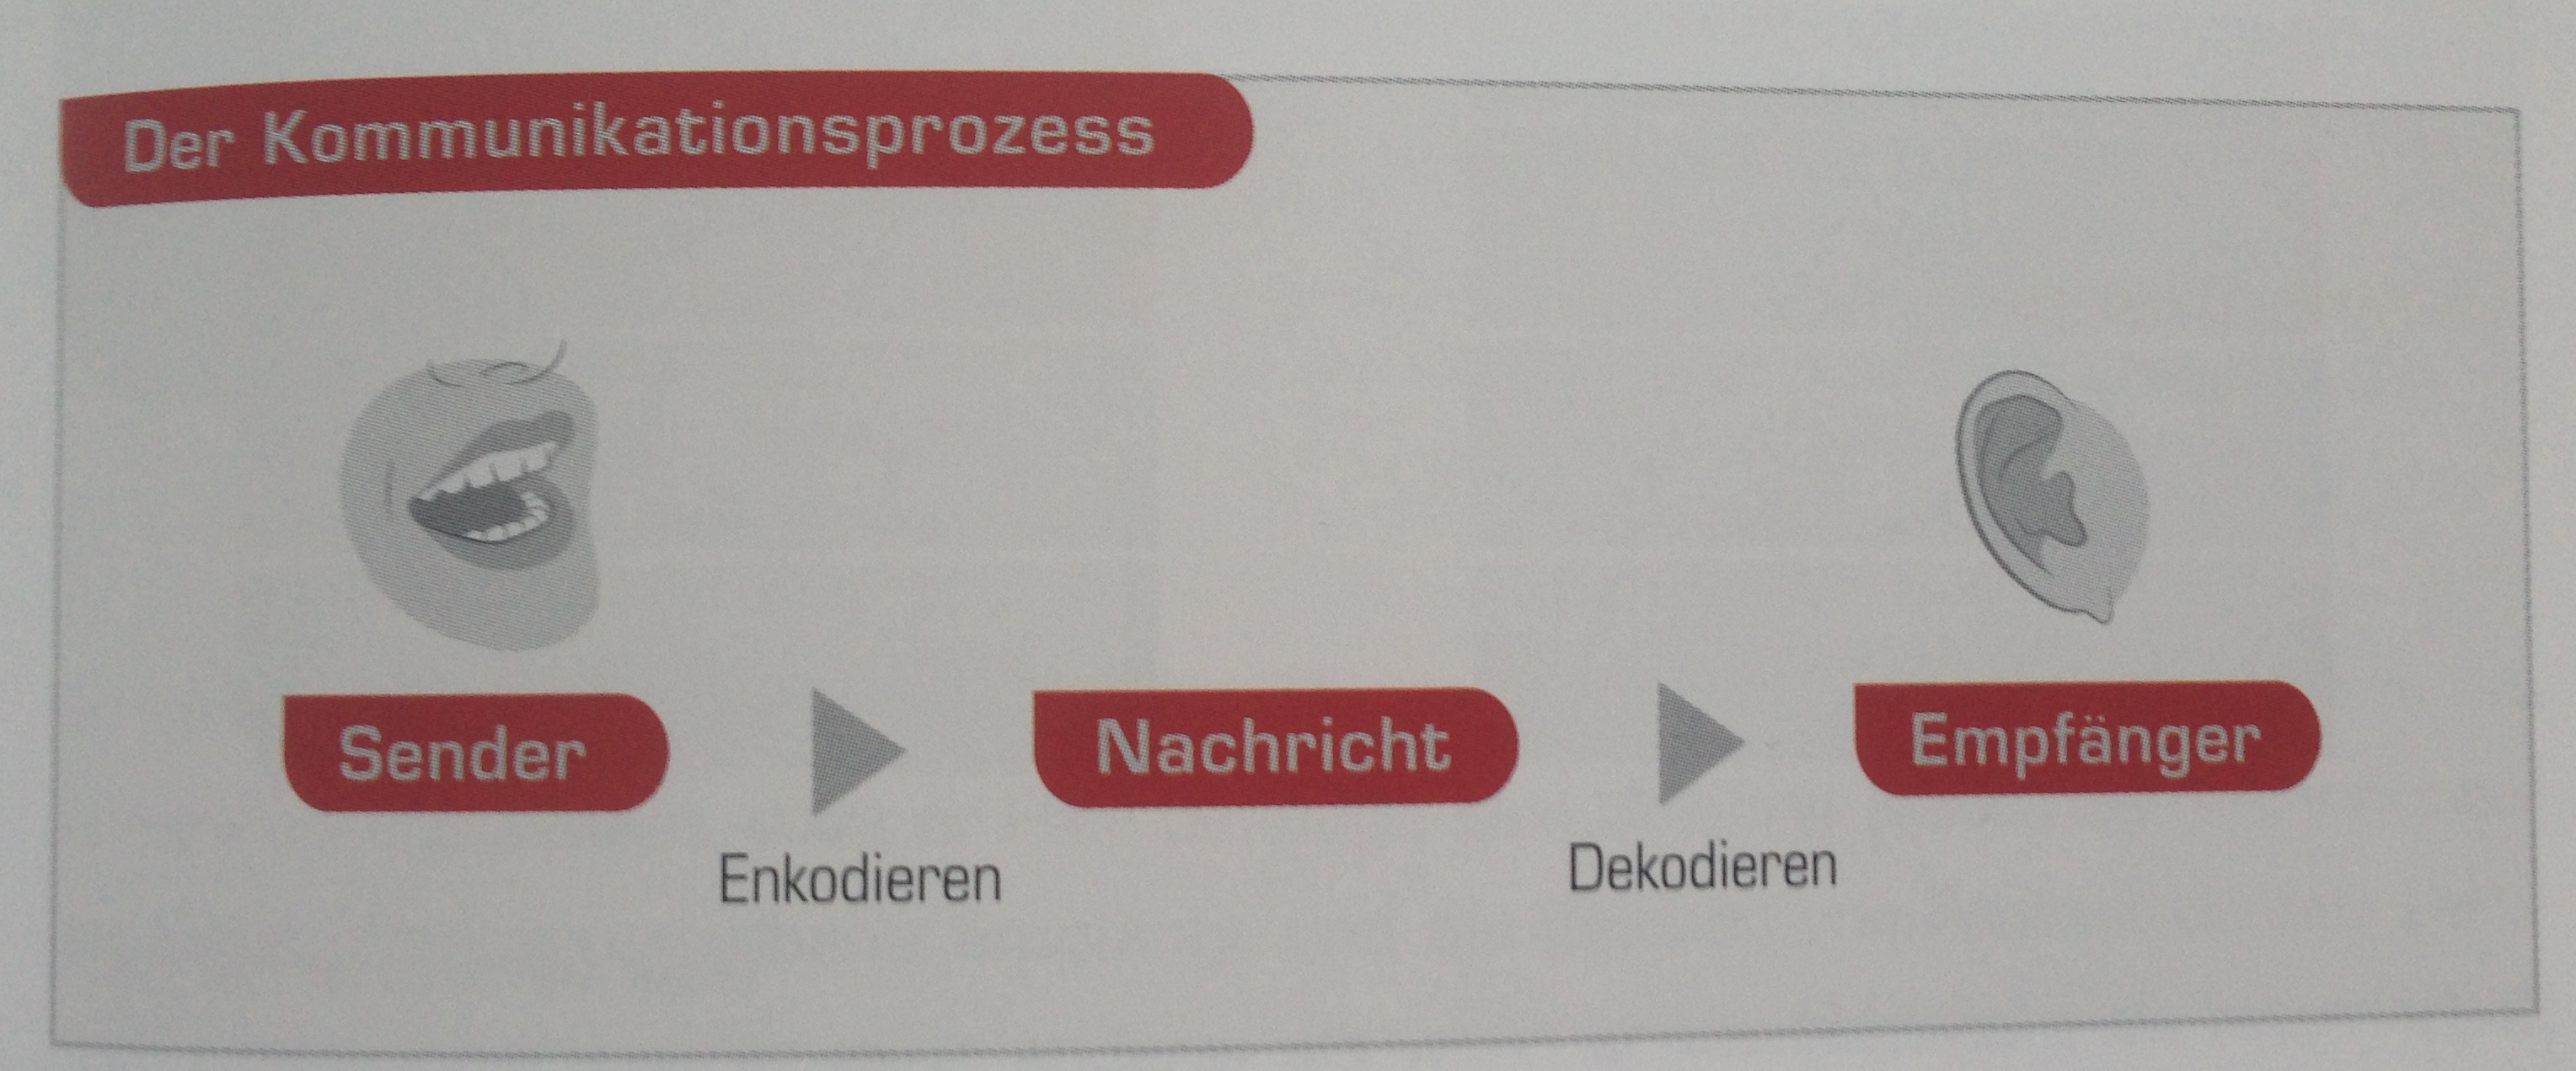
\includegraphics[width=12cm]{pic/kommunikation.jpg}
  \caption{Kommunikation.}
  \label{fig:kommunikation}
\end{figure}
\emph{Einflussfaktoren:}
\begin{itemize}
\item Aktuelle Stimmung und Emotionen
\item Erwartungen von Sender und Empfänger
\item Das gemeinsame Wissen (Verstehen Sender und Empfänger die gleichen Dinge unter den gleichen Begriffen?)
\item Aufmerksamkeit und Interesse
\item Zufällige Umstände
\item Störungen wie z.B. Wind oder Betrieb auf der Piste
\end{itemize}
\citetitle{theorie} Seite 251-252
\end{solution}

\begin{question}{6}
Beschreiben Sie das Vier-Ohren-Modell der Kommunikation anhand eines Beispiels aus dem Schneesport.
\end{question}
\begin{solution}
\begin{figure}[H]
  \centering
  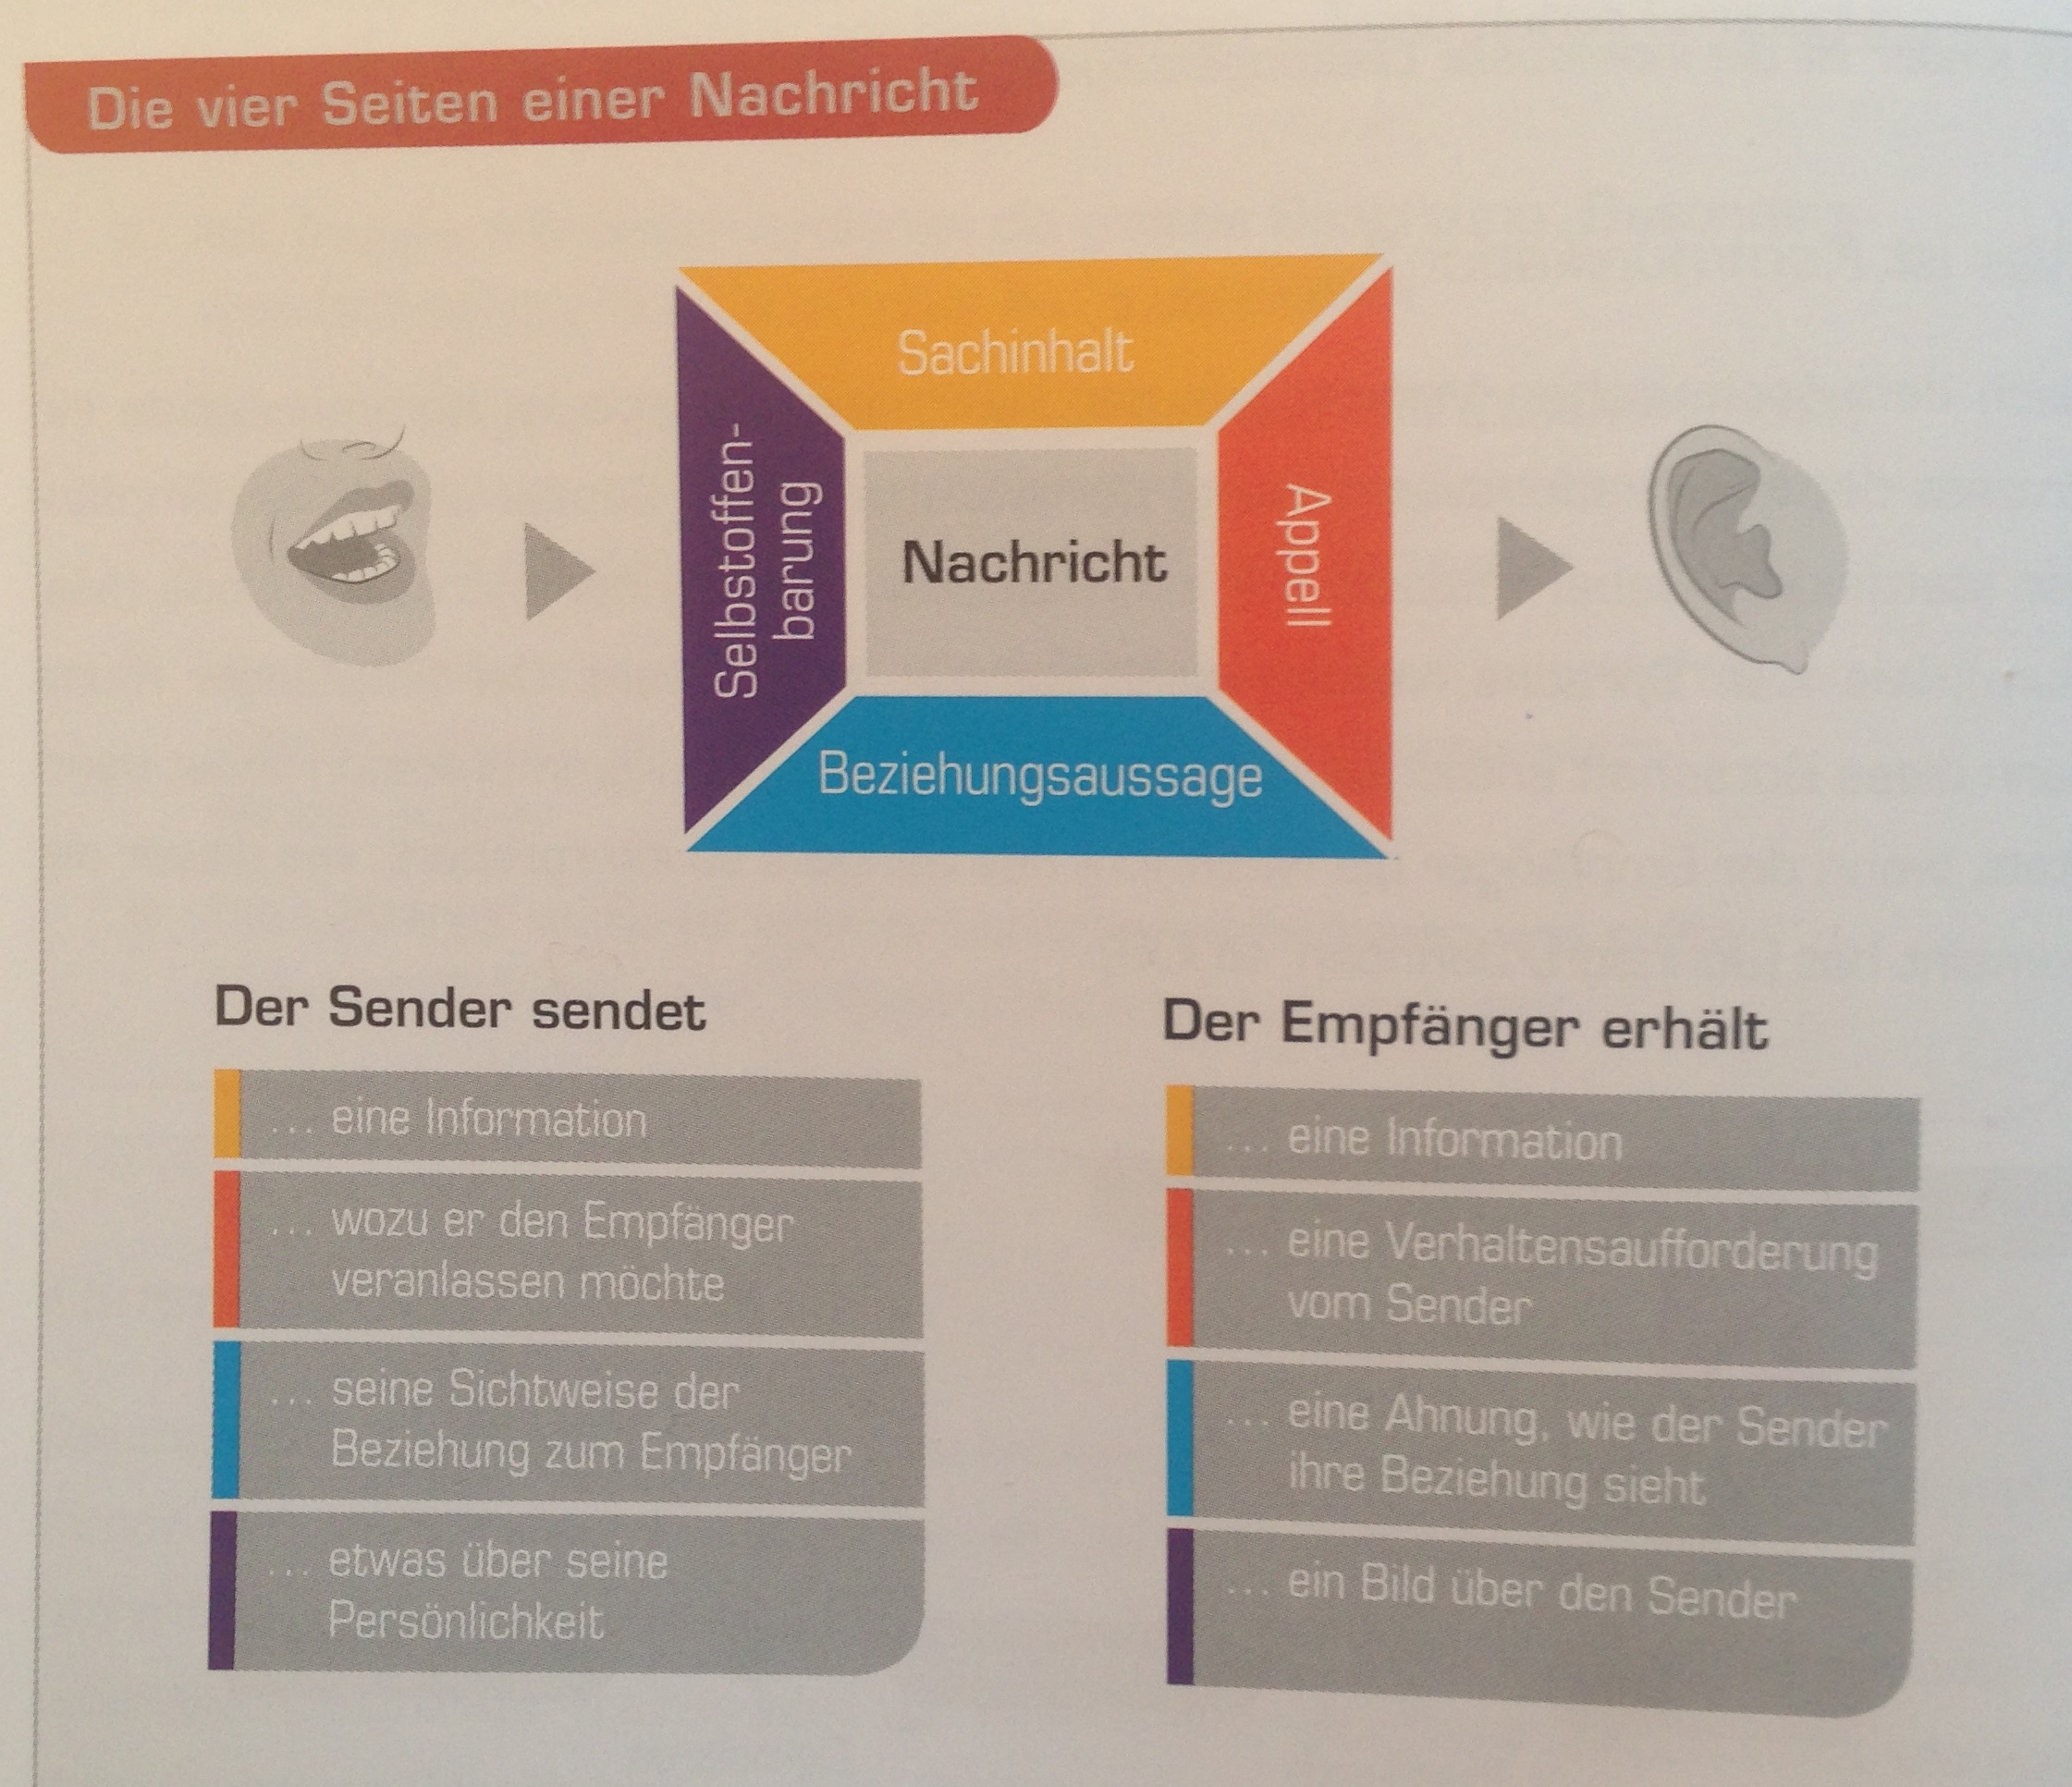
\includegraphics[width=12cm]{pic/vierohren.jpg}
  \caption{Vier Ohren Modell.}
  \label{fig:vierohren}
\end{figure}
\begin{figure}[H]
  \centering
  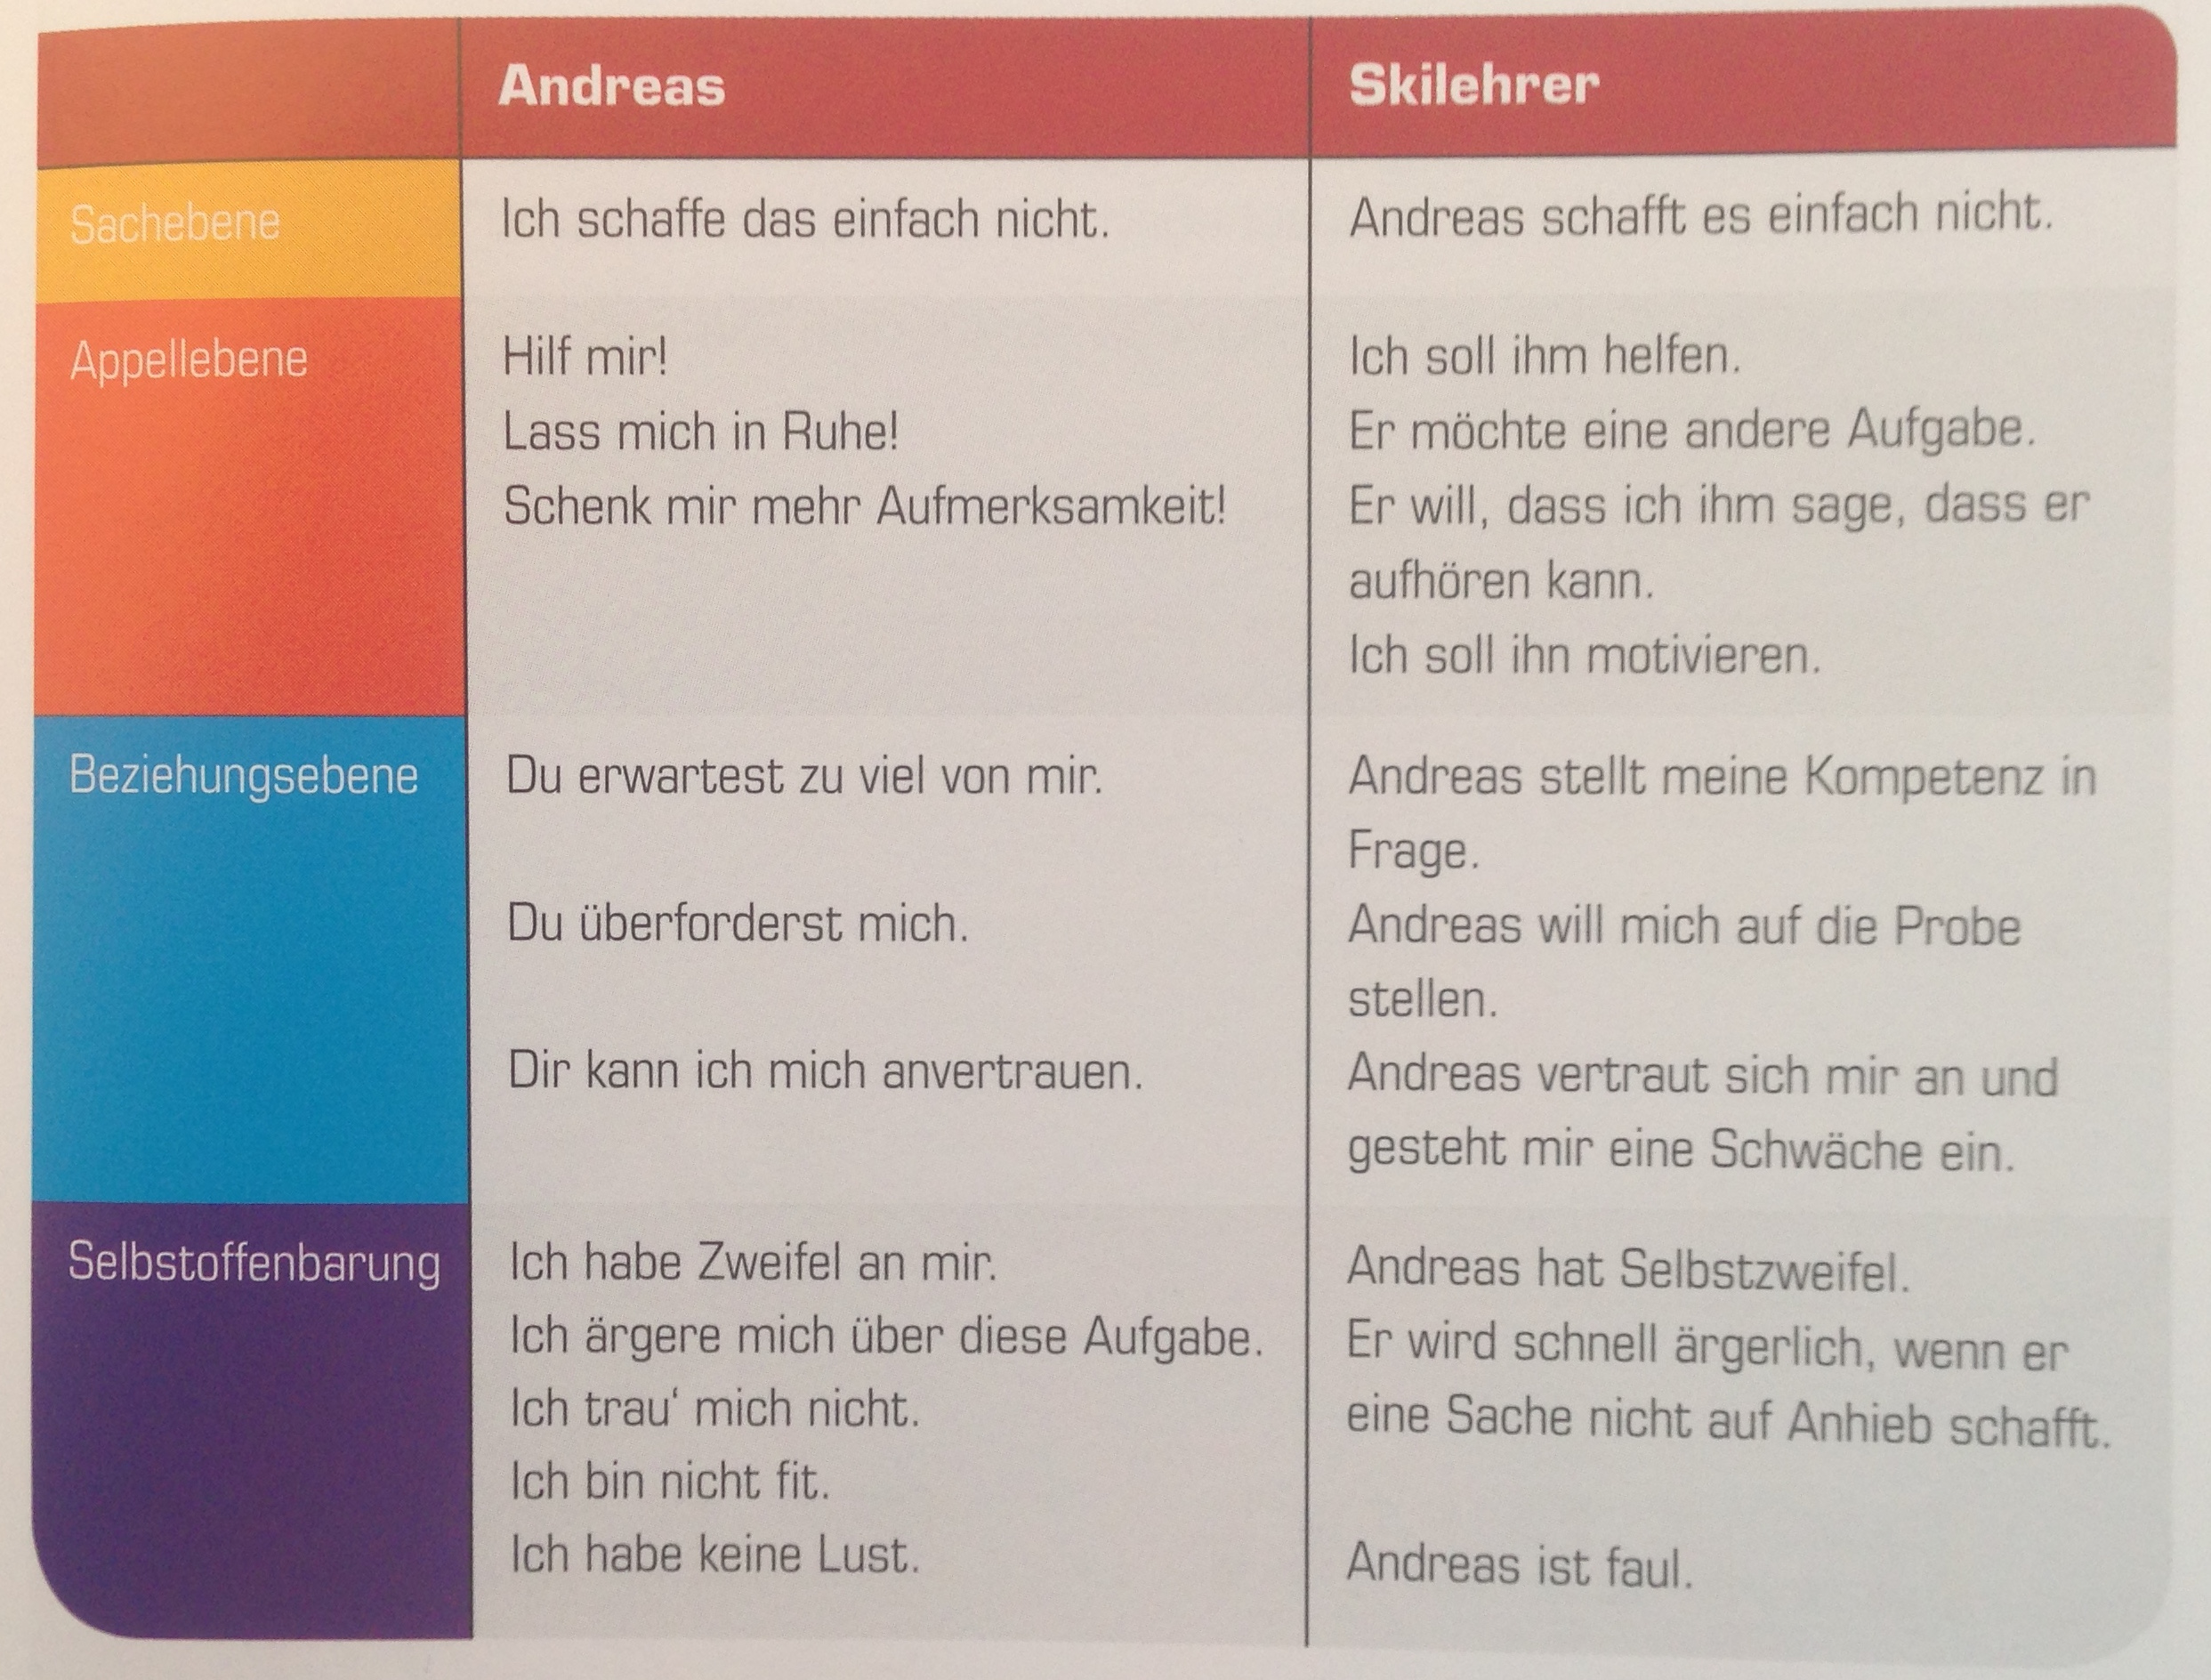
\includegraphics[width=12cm]{pic/vierohrenbsp.jpg}
  \caption{Beispiel.}
  \label{fig:viewrohrenbsp}
\end{figure}
\citetitle{theorie} Seite 252-253
\end{solution}

\begin{question}{6}
Als Schneesportlehrer müssen Sie für eine erfolgreiche Kommunikation aktiv Zuhören. Wie setzen Sie dies konkret im Unterricht um?
\end{question}
\begin{solution}
\begin{figure}[H]
  \centering
  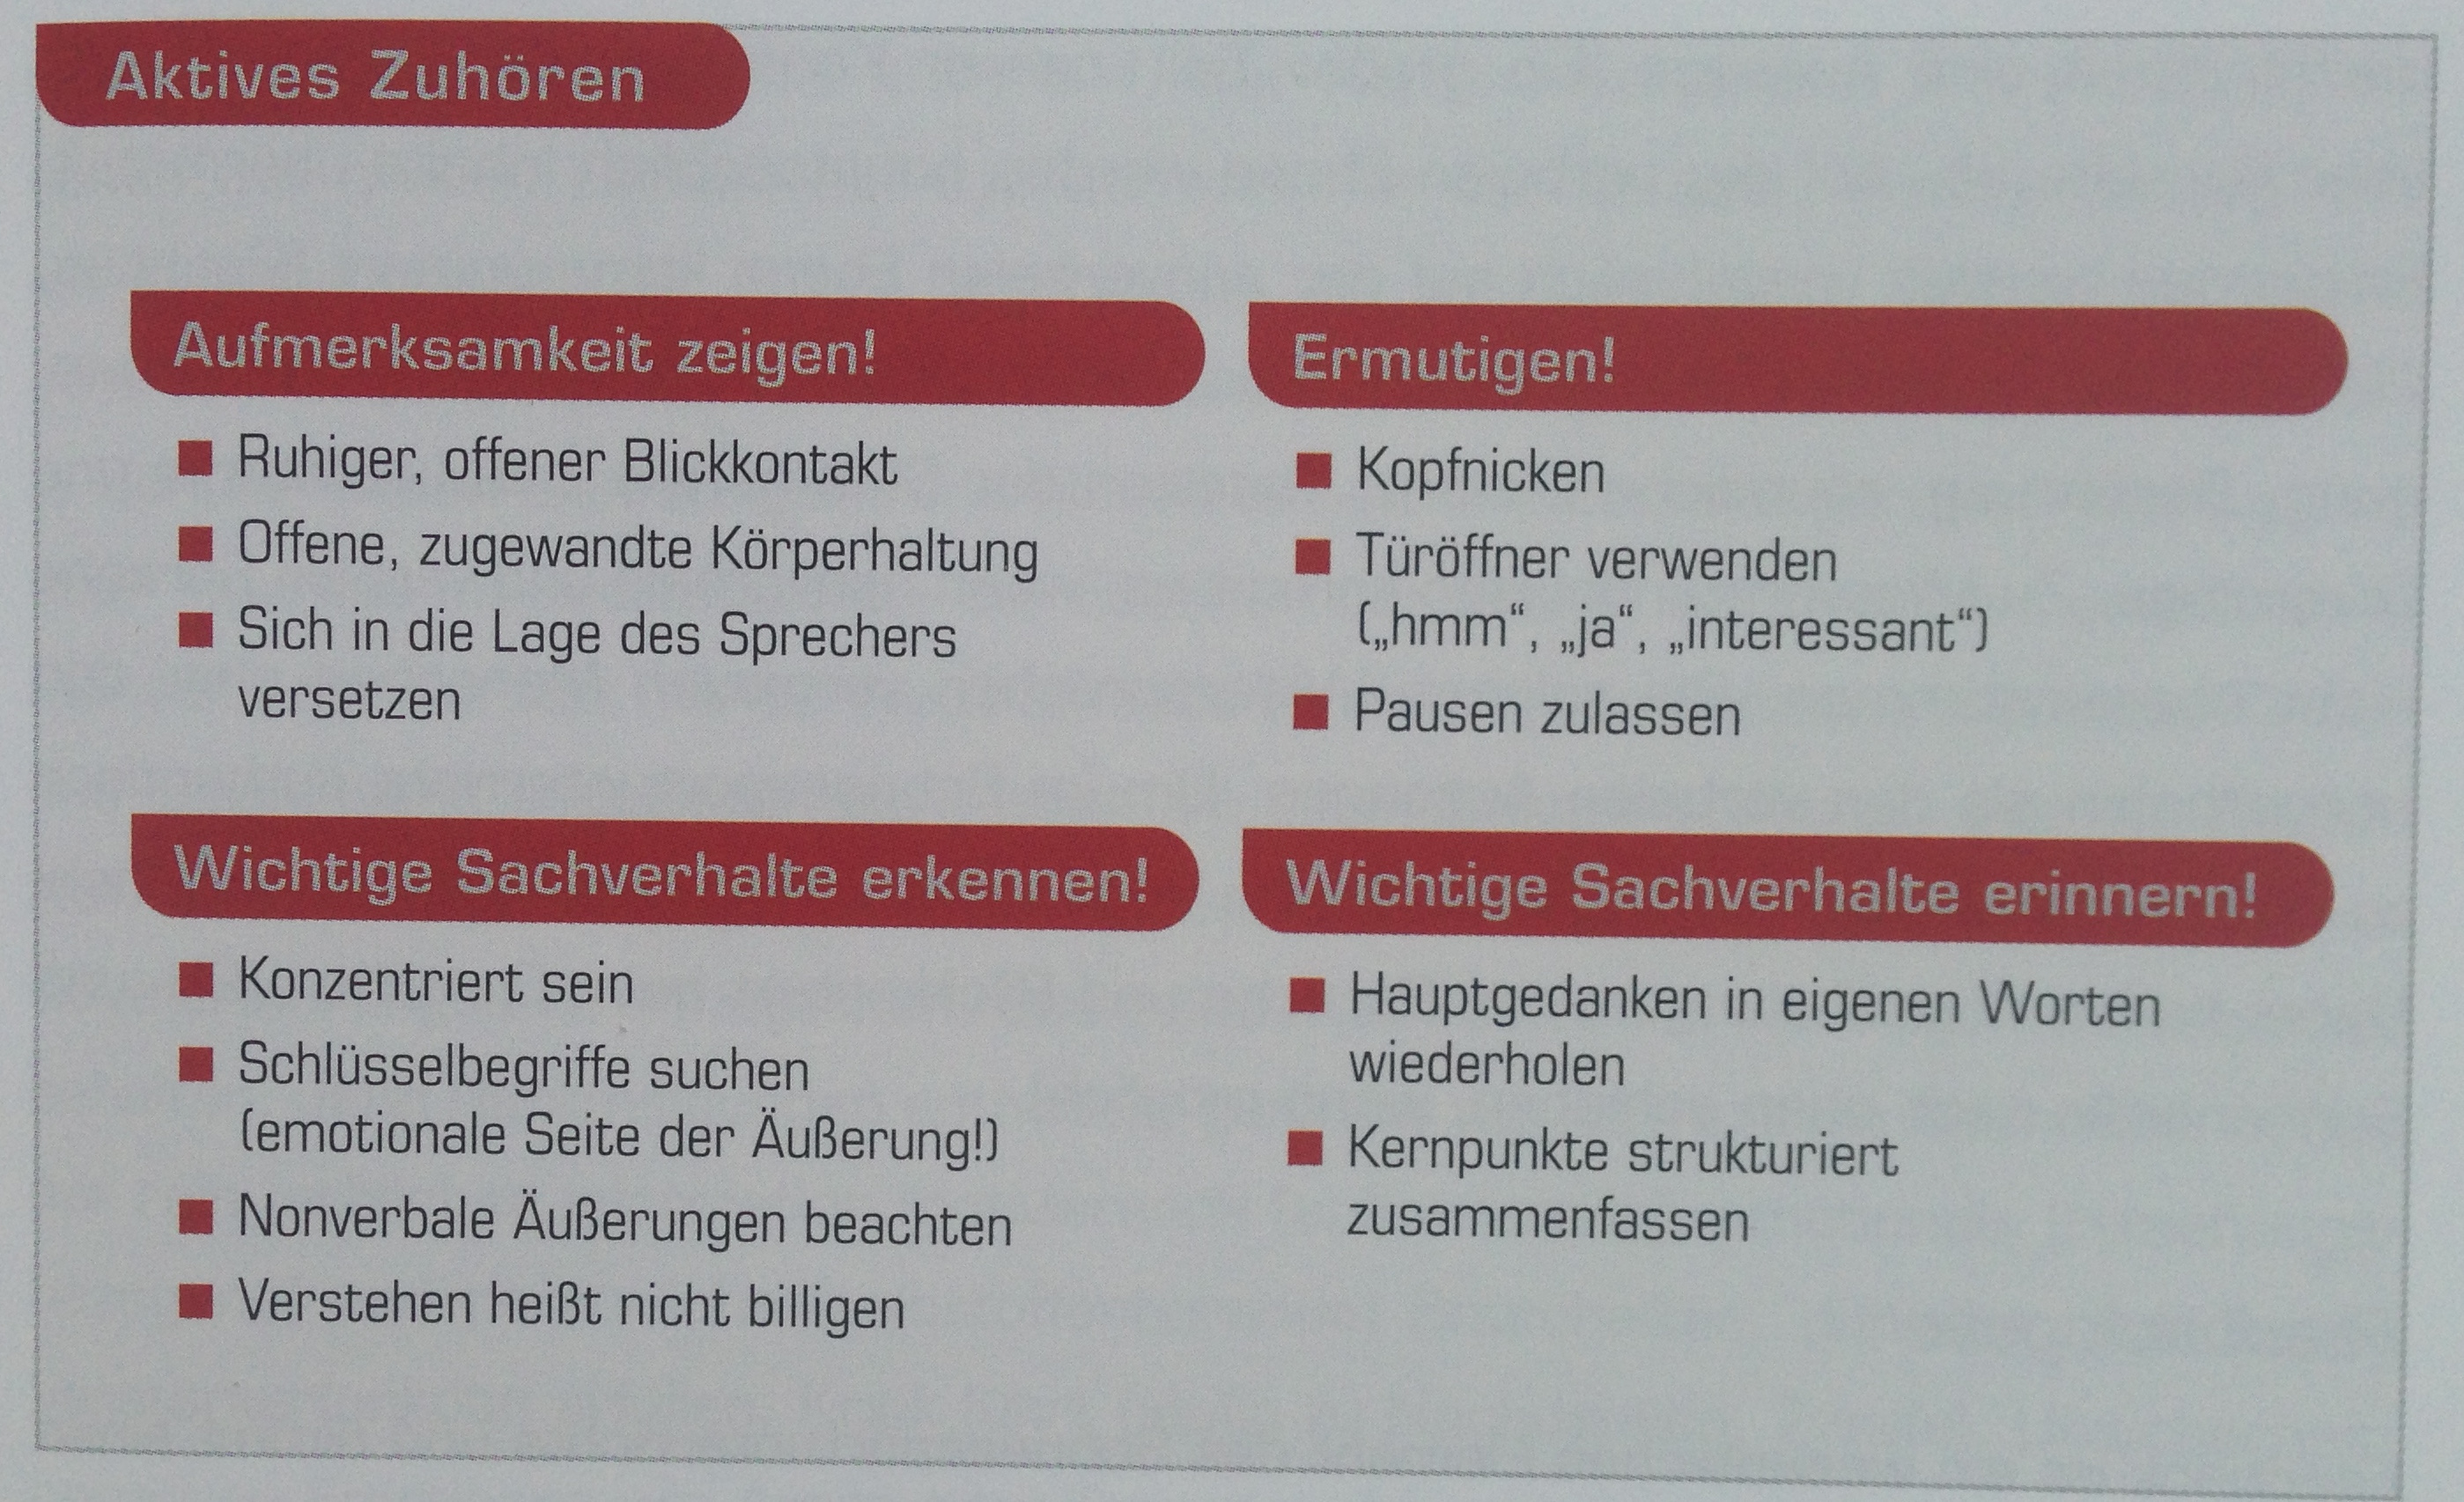
\includegraphics[width=12cm]{pic/zuhoeren.jpg}
  \caption{Aktives Zuhören.}
  \label{fig:zuhoeren}
\end{figure}
\citetitle{theorie} Seite 255
\end{solution}

\begin{question}{6}
Wie geben Sie Feedback an Ihre Schüler? Beschreiben Sie in diesem Zusammenhang fünf Feedbackregeln.
\end{question}
\begin{solution}
\emph{Feedbackregeln}
\begin{itemize}
\item Als persönliche Wahrnehmung in Ich-Form: „Ich habe gesehen, dass du rhythmisch und fließend gefahren bist.“, statt „Du fährst rhythmisch und fließend“
\item Situationsbezogen: „Bei dieser Fahrt hast du den Außenski wenig belastet.“, statt „Deine Außenskibelastung ist immer zu schwach.“
\item Beschreibend ohne Wertung: „Gerade bist du in Rückenlage gefahren“, statt „Du hängst hinten drin, das ist schlecht.“
\item Bezogen auf veränderbares Verhalten. Kritisiert wird nur das Verhalten, nicht die Person: „Du sprichst zu laut.“, statt „Du bist zu laut.“
\item An den Bedürfnissen des Schülers ausgerichtet: für Einsteiger häufiger, für Fortgeschrittene seltener
\item Immer mit einem positiven Aspekt beginnen.
\end{itemize}
\citetitle{theorie} Seite 257
\end{solution}

\begin{question}{5}
Warum können zwischen Lehrer und Schüler Probleme bei der Kommunikation auftreten? Welche Ursachen können hierfür grundsätzlich vorhanden sein?
\end{question}
\begin{solution}
\emph{Zwischen Kanälen:} Wenn Lehrer und Schüler auf unterschiedlichen Kanälen senden und Empfangen.\\
\emph{Innerhalb eines Kanals:} Beeinträchtigungen auf Beziehungsebene (Streit)\\
Störungen von Außen, Aufmerksamkeit, Interesse, Unterschiedliche Ausdrucksweise oder Sprache\\\\
\citetitle{theorie} Seite 252-257
\end{solution}

\begin{question}{4}
Definieren Sie den Begriff der Selbstwirksamkeit. Wie können Sie das Selbstvertrauen ihrer Schüler stärken? Geben Sie dazu drei Beispiele/ praktische Tipps.
\end{question}
\begin{solution}
\emph{Selbstwirksamkeit:} Selbstwirksamkeit ist der Glaube an die eigenen Fähigkeiten, eine bestimmte Aufgabe meistern zu können. Sie ist somit Aufgaben- und Situationsspezifisch und kann trainiert werden.\\
\emph{Stärkung der Selbstwirksamkeit:} 
\begin{itemize}
\item Persönliche Erfahrungen: Wiederholte Erfolgserlebnisse fördern das Selbstwirksamkeitserleben im Sport am besten.
\item Stellvertretende Erfahrungen: Das Betrachten eines anderen während der Bewegungsausführung steigert die Selbstwirksamkeitserwartung, und zwar umso mehr, je ähnlicher sich beide Personen in aufgabenrelevanten Eigenschaften sind. Auch die Imagination der eigenen Bewegung kann eine Quelle von mehr Selbstwirksamkeitserleben sein.
\item Verbale Überzeugung: Positive, auffordernde Sätze des Trainers, die dem Sportler Mut machen. Der Sportler kann auch lernen, sich selbst „gut zuzureden“, also sich selbst positive Instruktionen zu geben.
\item Emotionales Arousal: In welcher Gefühlslage wir uns befinden und v.a., wie wir dieses Gefühl (z.B. Angst) und die damit verbundenen körperlichen Zustände (z.B. Herzklopfen, Zittern) bewerten, kann sich stark auf unser Selbstvertrauen auswirken.
\end{itemize}
\citetitle{theorie} Seite 264-266
\end{solution}

\begin{question}{6}
Beschreiben Sie den Teufelskreis der Angst.
\end{question}
\begin{solution}
\begin{figure}[H]
  \centering
  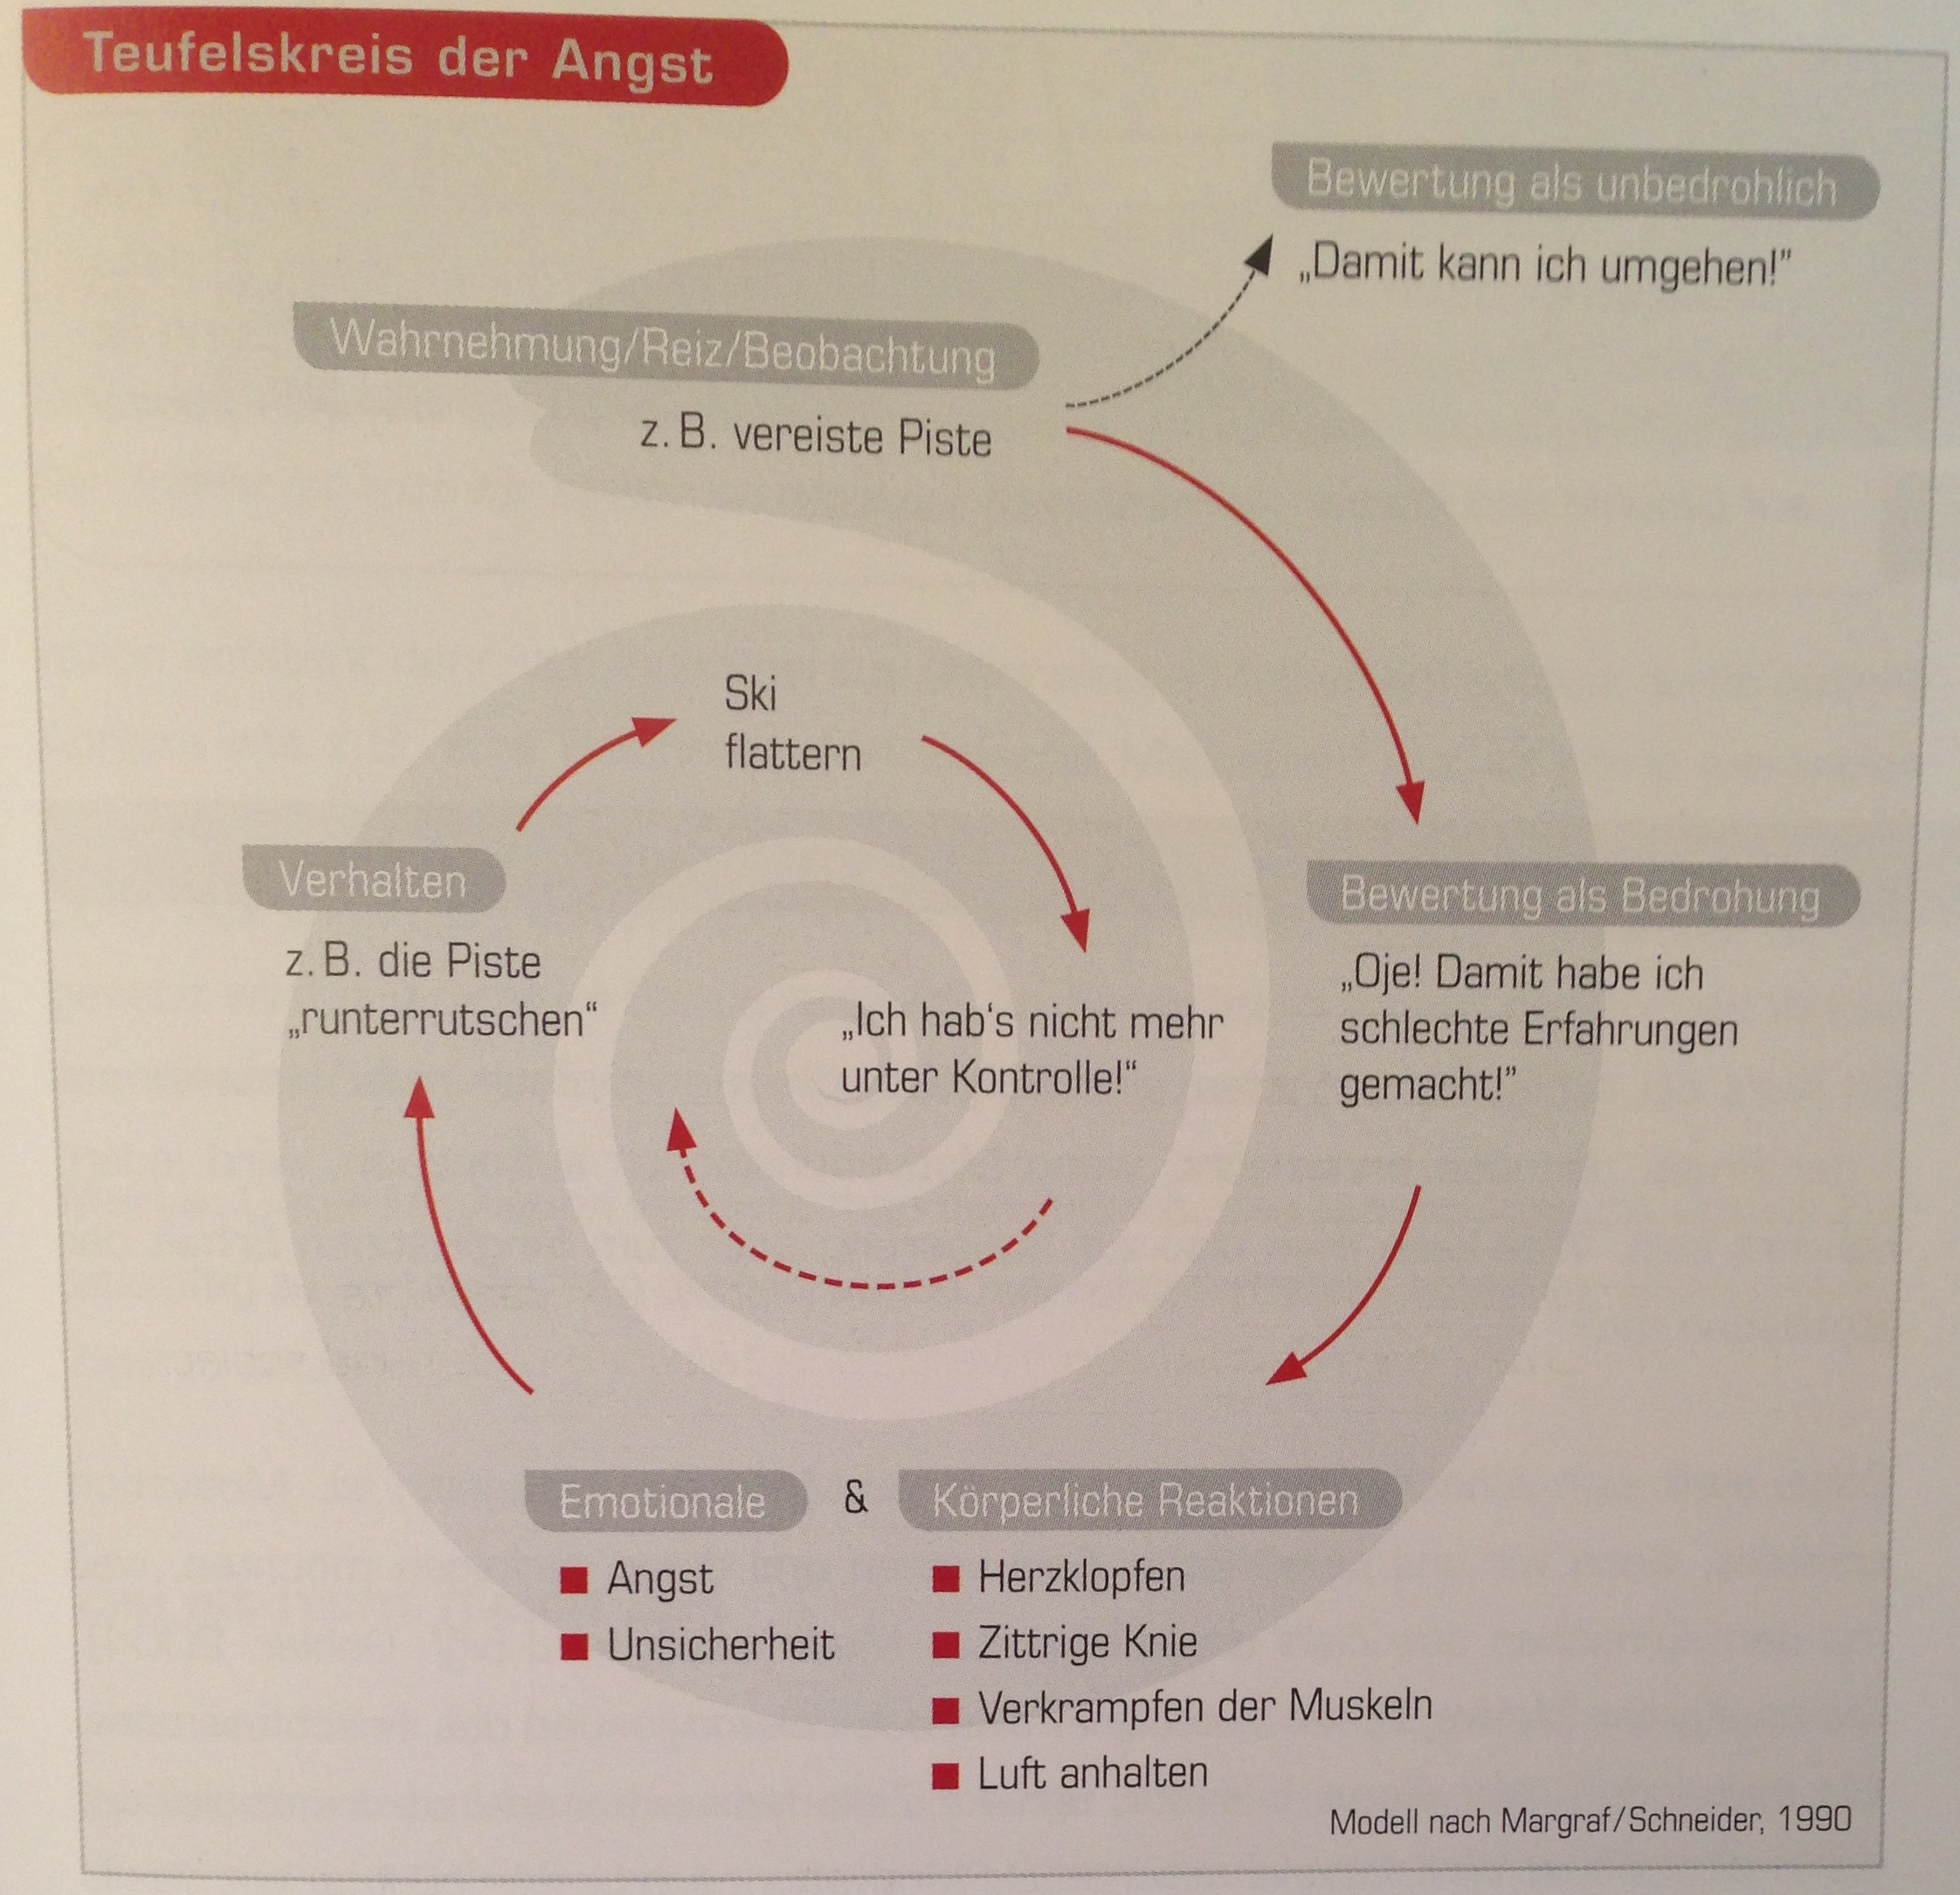
\includegraphics[width=12cm]{pic/angst.jpg}
  \caption{Teufelskreis der Angst.}
  \label{fig:angst}
\end{figure}
Was passiert, wenn jemand keine Selbstwirksamkeitserwartung aufbaut und sich z. B. steile Abfahrten, Tiefschneefahrten oder Wettkämpfe nicht zutraut? Angst macht sich breit und das bereits Gelernte ist viel schlechter abrufbar. Der Schüler wird die Aufgabe nicht so gut meistern, wie er es aufgrund seiner technischen Fertigkeiten kötinnte. Am Teufelskreis der Angst von Margraf und Schneider (1990) wird deutlich, wie sehr Gefühle. Gedanken und Verhalten zusammenhängen und sich aufschaukeln können und wo man eingreifen kann, um der lch-kann-nichtc-Falle zu entkommen.\\\\
\citetitle{theorie} Seite 267
\end{solution}

\begin{question}{2}
Nennen Sie vier Entspannungsverfahren, die in der Sportpsychologie angewendet werden.
\end{question}
\begin{solution}
\begin{itemize}
\item 
\end{itemize}
\citetitle{theorie} Seite 267
\end{solution}